
\subsection{実験の目的,概要}
1桁のBCDコードを出力するBCDカウンタを設計し,それをもとに2桁のBCDコード出力するBCDカウンタを階層設計によって設計する。
設計した2つの回路で,それぞれ機能レベルシュミレーションと論理合成を実行し,入出力の正しさと合成による結果を確認する。

ICE計算機上の,ModelSim,Quartusを使用する。

この実験で,簡単な順序回路の設計方法と,それをもとにした階層設計の方法を実践し,習得することを目的にする。

\subsection{実験方法}
\subsection*{課題1-1}
\subsubsection{回路のHDL記述}
以下のような回路記述をbcd1.v,テストベンチをtest\_bcd1.vとして作成した。
\lstinputlisting[caption=bcd1.v,label=bcd1.v]{./src/bcd/bcd1.v}
\lstinputlisting[caption=test\_bcd1.v,label=testbcd1.v]{./src/bcd/test_bcd1.v}

\subsubsection{機能レベルシュミレーション}
作成したテストベンチをもとに,ModelSimで信号波形を出力した。
入出力の値が仕様通りの真理値表と一致することを確認した。

\subsubsection{論理合成}
以下の2ファイルを作成し,配置した。
\lstinputlisting[caption=bcd1.qpf,label=bcd1.qpf]{./src/bcd/bcd1.qpf}
\lstinputlisting[caption=bcd1.qsf,label=bcd1.qsf]{./src/bcd/bcd1.qsf}

作成した回路記述をQuartusでコンパイルし,論理合成とレイアウトを行した。
回路構成やロジックエレメント数,遅延時間について確認した。

\subsection*{課題1-2}
以下のような回路記述をbcd2.v,テストベンチをtest\_bcd2.vとして作成した
\lstinputlisting[caption=bcd2.v,label=bcd2.v]{./src/bcd/bcd2.v}
\lstinputlisting[caption=test\_bcd2.v,label=testbcd2.v]{./src/bcd/test_bcd2.v}

\subsubsection{機能レベルシュミレーション}
作成したテストベンチをもとに,ModelSimで信号波形を出力した。
入出力の値が仕様通りの真理値表と一致することを確認した。

\subsubsection{論理合成}
以下の2ファイルを作成し,配置した。
\lstinputlisting[caption=bcd2.qpf,label=bcd2.qpf]{./src/bcd/bcd2.qpf}
\lstinputlisting[caption=bcd2.qsf,label=bcd2.qsf]{./src/bcd/bcd2.qsf}

作成した回路記述をQuartusでコンパイルし,論理合成とレイアウトを行った。
回路構成やロジックエレメント数,遅延時間について確認した。

\subsection{実験結果}
\subsection*{課題1-1}
\subsubsection{機能レベルシュミレーション}
ModelSimで波形を作成した結果,以下のような波形になった。

\begin{figure}[H]
  \centering
  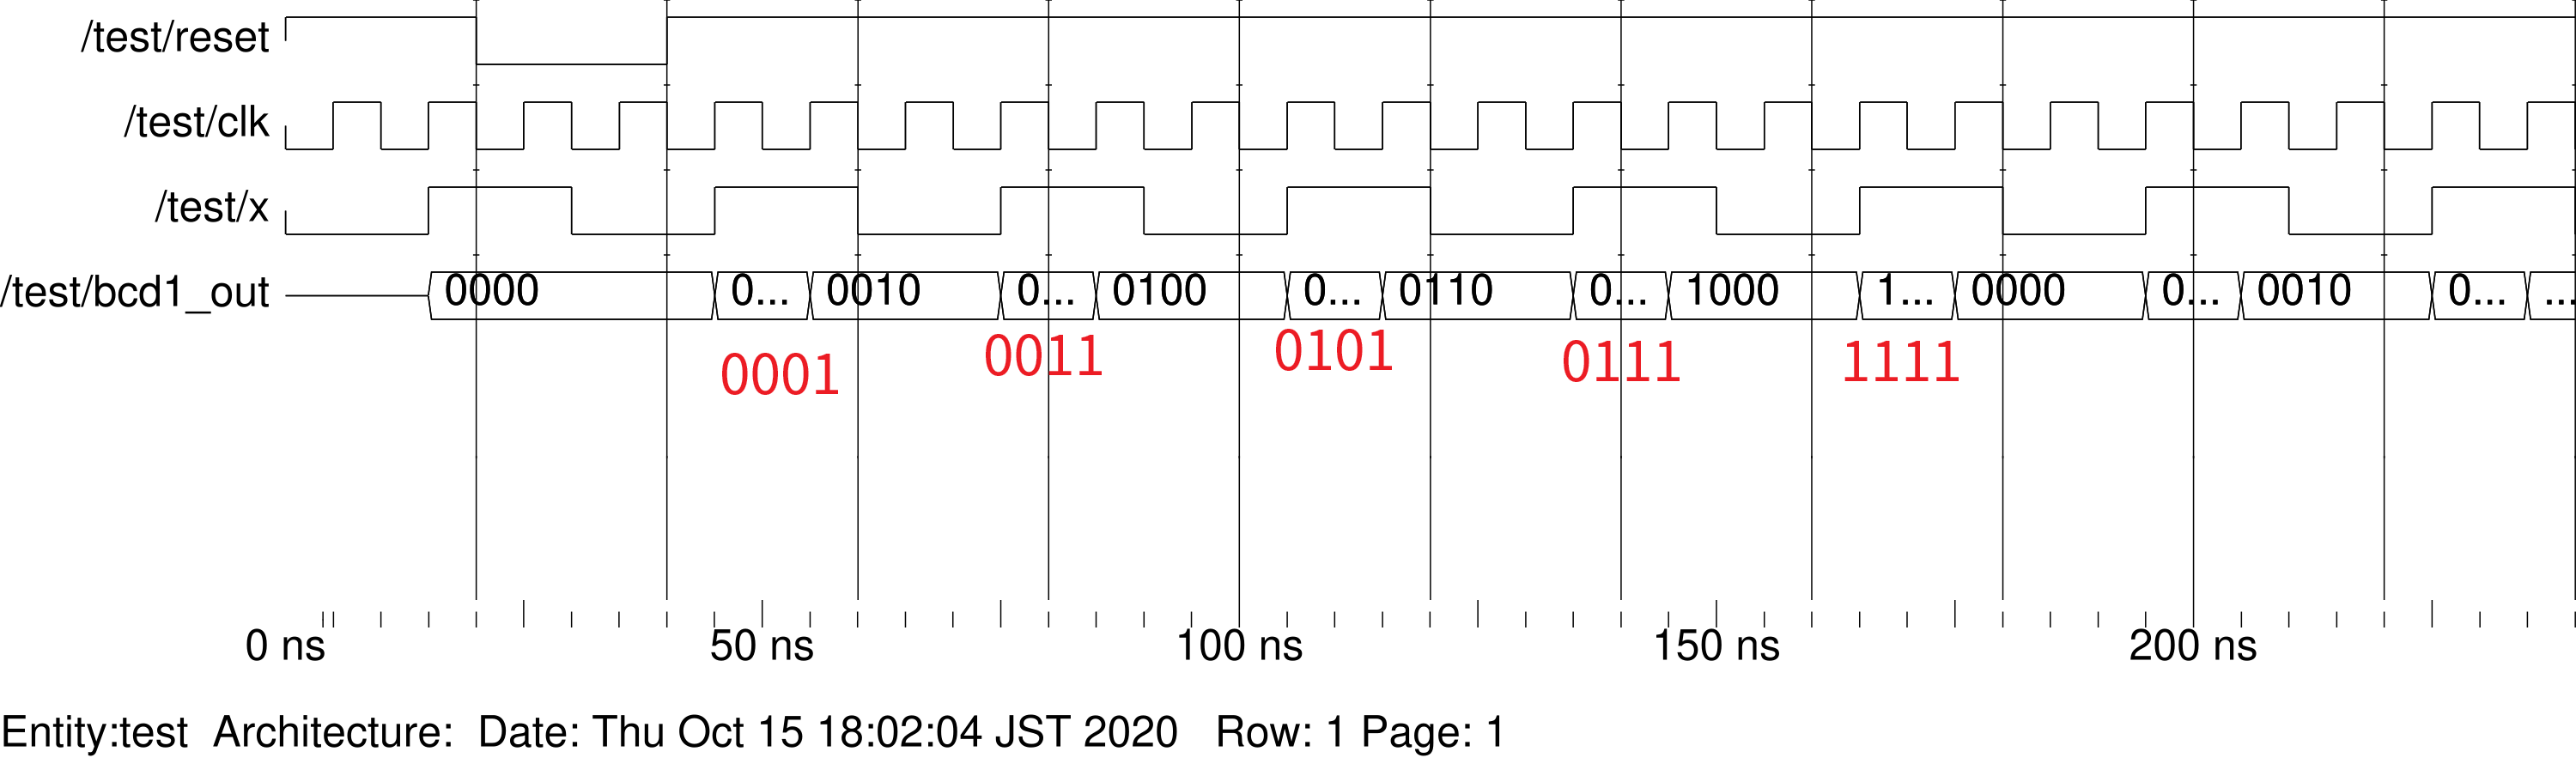
\includegraphics[width=\linewidth]{./src/bcd/bcd1wave.png}
  \caption{bcd1の波形}
\end{figure}

bcd1\_outの値は期待通り10進1桁bcdカウンタとして機能している。

\subsubsection{論理合成}
論理合成の結果,以下のような回路が作られた。

\begin{figure}[H]
  \centering
  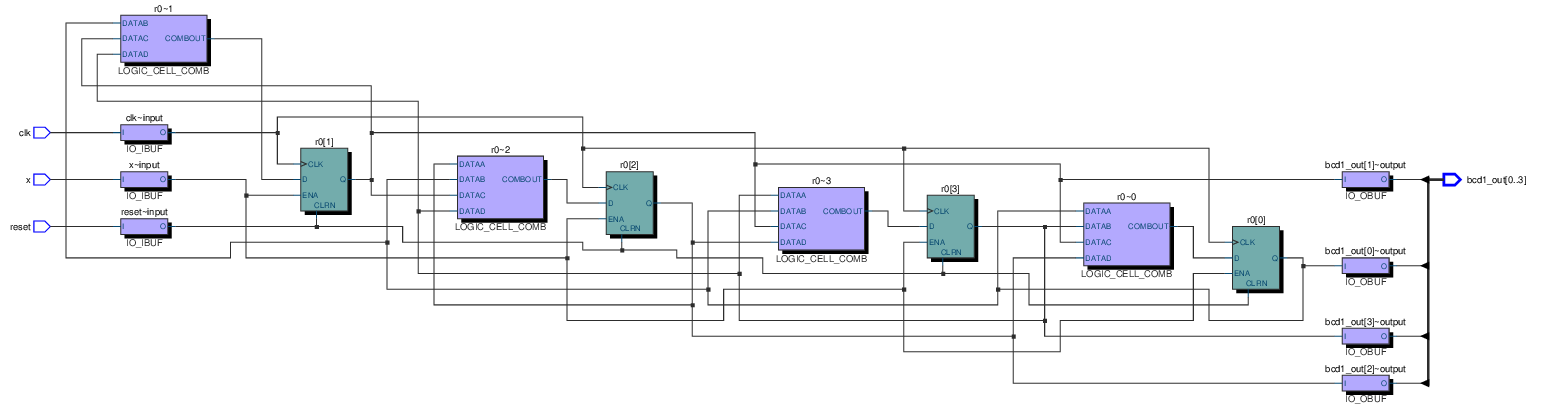
\includegraphics[width=\linewidth]{./src/bcd/bcd1surc.png}
  \caption{bcd1の回路}
\end{figure}

ロジックエレメント数は5だった。

回路全体の遅延時間は,以下のようになった。

\begin{figure}[H]
  \centering
  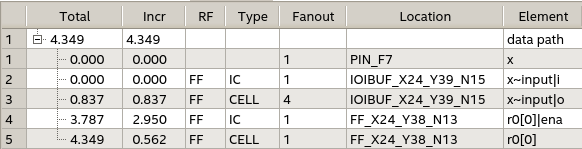
\includegraphics[width=\linewidth]{./src/bcd/bcd1timing.png}
  \caption{bcd1の遅延時間}
\end{figure}

\subsection*{課題1-2}
\subsubsection{機能レベルシュミレーション}
ModelSimで波形を作成した結果,以下のような波形になった。

\begin{figure}[H]
  \centering
  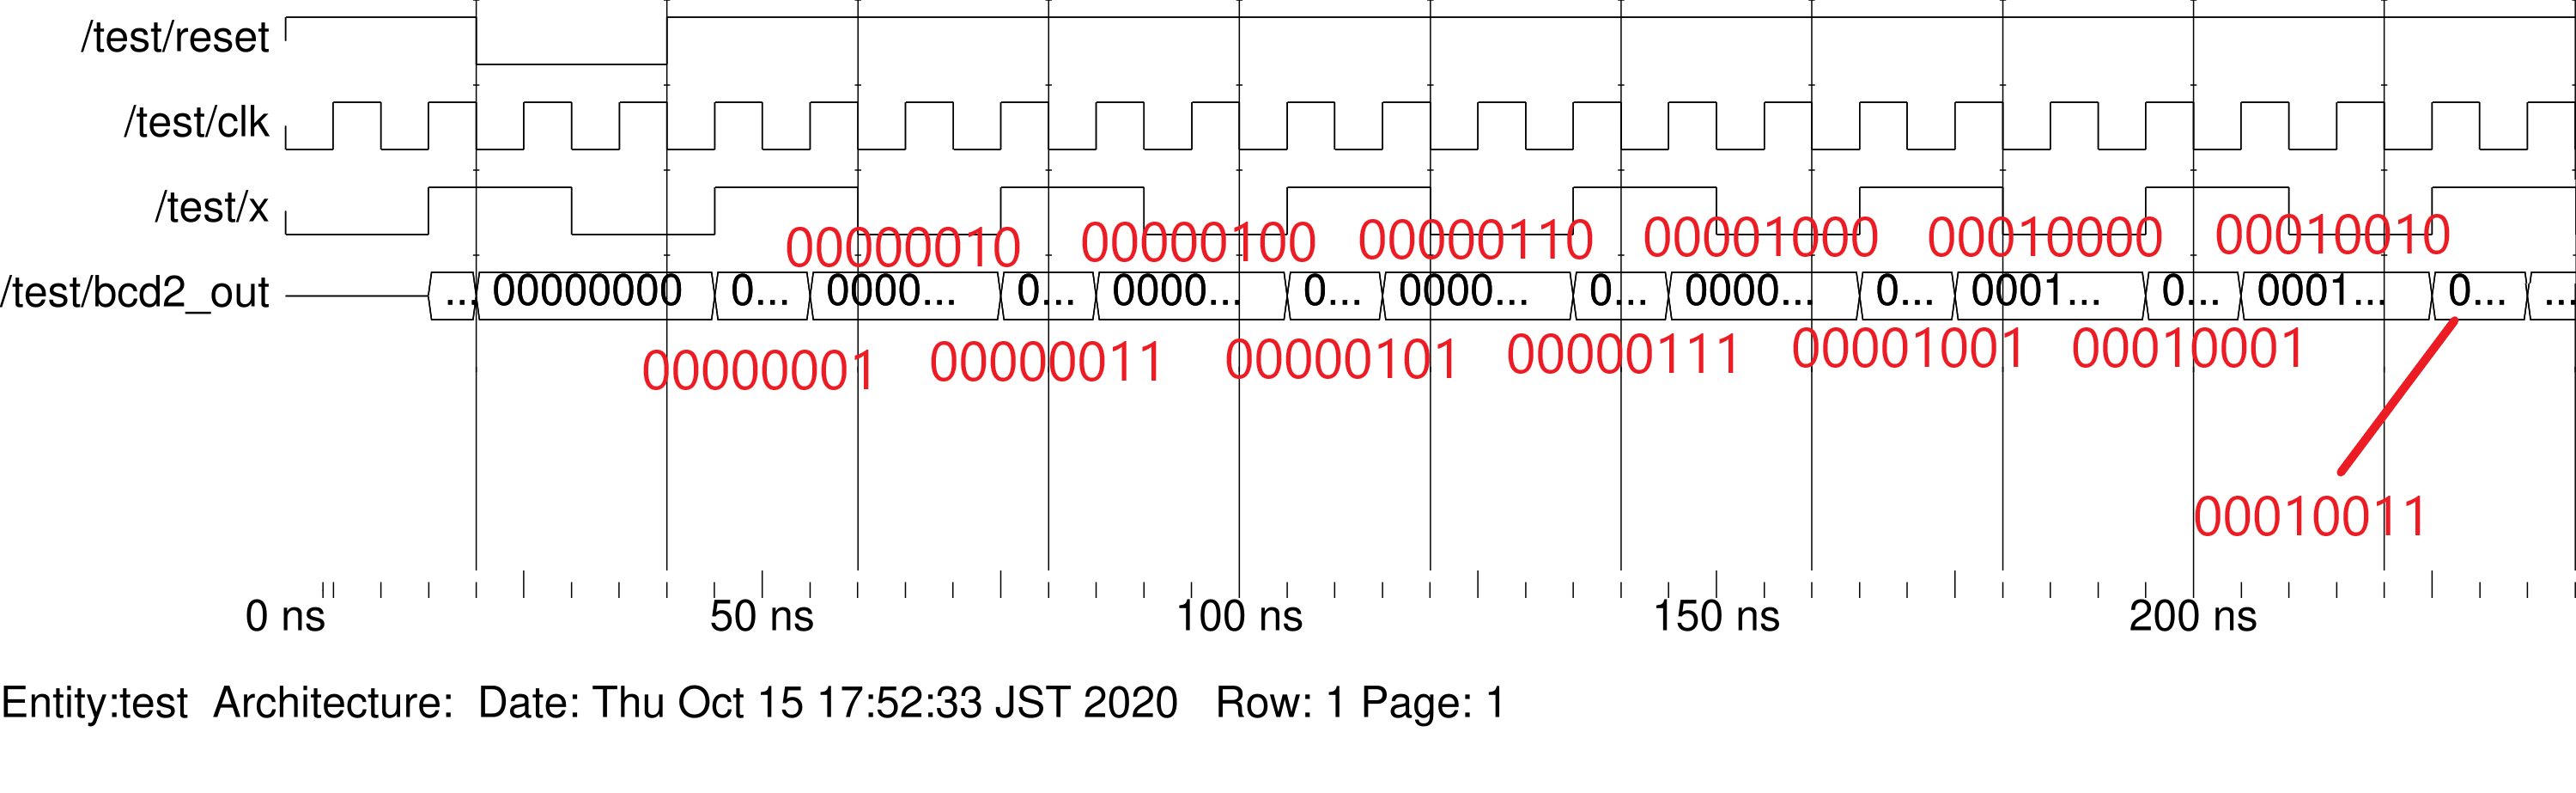
\includegraphics[width=\linewidth]{./src/bcd/bcd2wave.png}
  \caption{bcd2の波形}
  \label{bcd2の波形}
\end{figure}

bcd1\_outの値は期待通り10進2桁bcdカウンタとして機能している。

\subsubsection{論理合成}
論理合成の結果,以下のような回路が作られた。

\begin{figure}[H]
  \centering
  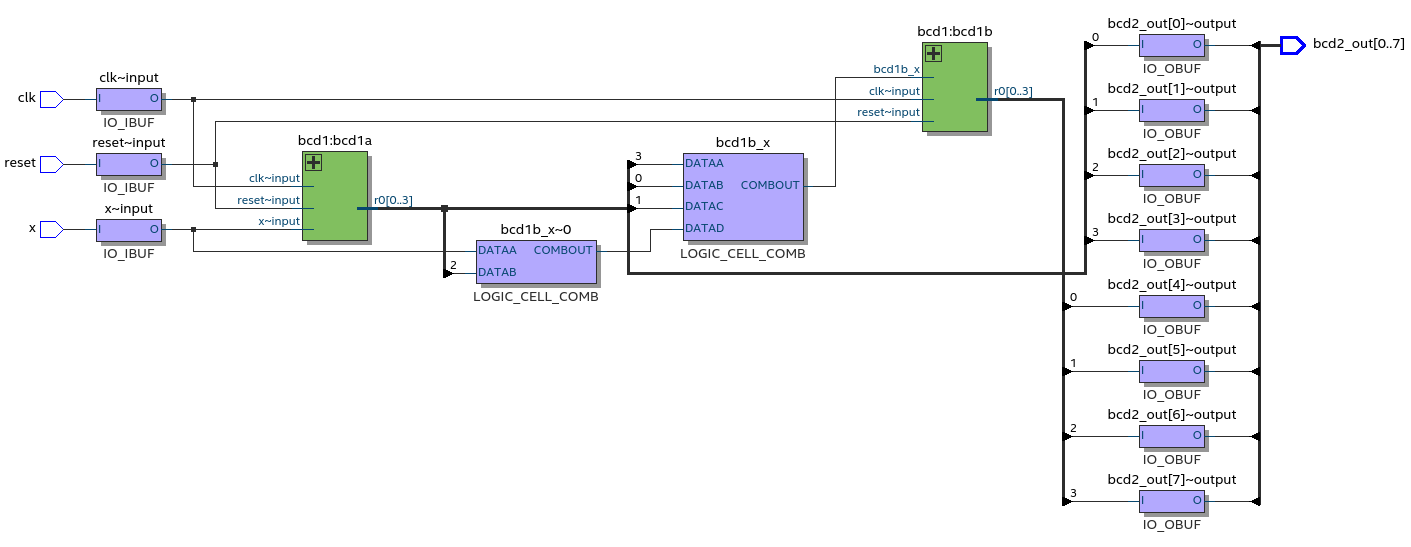
\includegraphics[width=\linewidth]{./src/bcd/bcd2surc.png}
  \caption{bcd2の回路}
  \label{bcd2の回路0}
\end{figure}

bcd1モジュールの他に以下のゲート構成があった。

\begin{figure}[H]
  \centering
  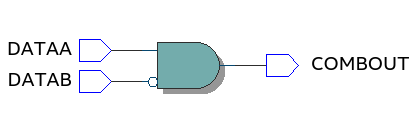
\includegraphics[width=\linewidth]{./src/bcd/bcd2-2x.png}
  \caption{xとbcd1a[2]}
  \label{bcd2の回路1}
\end{figure}

\begin{figure}[H]
  \centering
  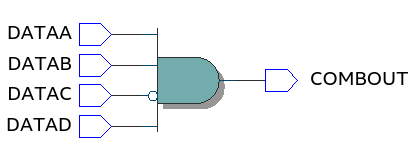
\includegraphics[width=\linewidth]{./src/bcd/bcd2031.png}
  \caption{bcd2[3,0,1]}
  \label{bcd2の回路2}
\end{figure}

ロジックエレメント数は11だった。

回路全体の遅延時間は,以下のようになった。

\begin{figure}[H]
  \centering
  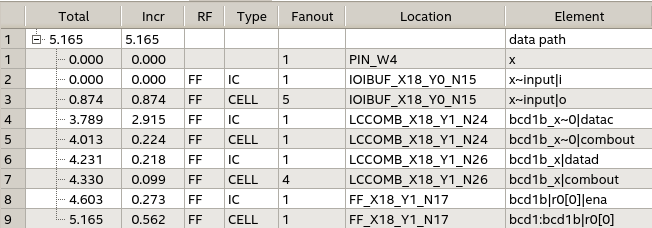
\includegraphics[width=\linewidth]{./src/bcd/bcd2timing.png}
  \caption{bcd2の遅延時間}
\end{figure}

\subsection{考察}
\subsection*{課題1-1}
\subsubsection{回路のHDL記述}
コード\ref{bcd1.v}ではクロックの立ち上がりで,x=1のときに限ってインクリメントしている。
また,レジスタの値が9以上ならば,ゼロを代入している。

リセット信号は,立ち下がりでレジスタにゼロを代入している。

テストベンチ(コード\ref{testbcd1.v})では,5nsごとのクロック反転と,15nsごとのxの反転を実行している。

また,開始20ns後から40ns後までリセット信号を0にしている。

\subsubsection{機能レベルシュミレーション}
1桁のbcdカウンタとして,クロックとxの値によって0~9までの値をとっていた。

\subsubsection{論理合成}
回路では,4桁分のレジスタ用フリップフロップと,各桁での論理演算回路が4桁分あることがわかる。

\subsection*{課題1-2}
\subsubsection{回路のHDL記述}
コード\ref{bcd2.v}では,bcd1のモジュールを利用して2桁分のBCDカウンタを実現している。
具体的には,1桁目が9で桁上りするときに限って,2桁目のBCDカウンタにxを入力している。
また,クロック信号は2つのモジュールに同じ信号を与えている。

リセット信号は,立ち下がりで2つのbcd1モジュールにリセット信号を入力している。

テストベンチ(コード\ref{testbcd2.v})では,5nsごとのクロック反転と,15nsごとのxの反転を実行している。

また,開始20ns後から40ns後までリセット信号を0にしている。

\subsubsection{機能レベルシュミレーション}
図\ref{bcd2の波形}より,4bitを10進1桁分として,2桁分のBCDカウンタが動作している。

\subsubsection{論理合成}
合成された回路では,1桁目の2bit目とxをとって演算した結果を,他のbitと合成して,2桁目のxとして入力していることがわかる。
この部分が,$(bcd1a\_out == 1001) \land x$の結果として反映されていることが分かった。
ほとんど設計したとおりにモジュールが配置されている。

このとき,bcd1モジュールをインラインで展開した場合,回路の構成が異なる可能性がある。
今回の結果より,モジュールの中身については各モジュールで最適化したのと同じ最適化が施されている。
よって,階層設計による回路よりも,インラインで記述したほうがロジックエレメント数や,遅延時間が改善する可能性がある,と予想される。
今回の実験ではわからなかったが,もしそのような差異があるならば,ボード規模などの制限によっては,記述しやすい階層設計と,インラインの記述を使い分ける必要があると予想した。\\

この実験で,順序回路の階層設計の手法と,階層化によって論理合成がどのように行われるかについて理解できた。
